
%% XXXXXX Questions used on the
%% NYSED Physics Regents Examination
%%--------------------------------------------------

%% this section contains XX problems


%% Section June2016
%%--------------------
\element{nysed}{
\begin{question}{June2016-Q02}
    A \SI{65.0}{\kilo\gram} astronaut weighs \SI{638}{\newton} at the surface of Earth. 
    What is the mass of the astronaut at the surface of the Moon,
        where the acceleration due to gravity is \SI{1.62}{\meter\per\second\squared}?
    \begin{multicols}{2}
    \begin{choices}
        \wrongchoice{\SI{10.7}{\kilo\gram}}
      \correctchoice{\SI{65.0}{\kilo\gram}}
        \wrongchoice{\SI{105}{\newton}}
        \wrongchoice{\SI{638}{\newton}}
    \end{choices}
    \end{multicols}
\end{question}
}

\element{nysed}{
\begin{question}{June2016-Q09}
    The diagram below represents the path of a thrown ball through the air.
    \begin{center}
    \begin{tikzpicture}
        %% NOTE: TODO: diagram
    \end{tikzpicture}
    \end{center}
    Which arrow best represents the direction in which friction acts on the ball at point $P$?
    \begin{multicols}{2}
    \begin{choices}
        \AMCboxDimensions{down=-0.3cm}
        \wrongchoice{
            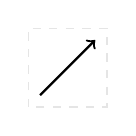
\begin{tikzpicture}
                \draw[white!90!black,dashed] (0,0) rectangle (1,1);
                \draw[thick,->] (0.15,0.15) -- (0.85,0.85);
            \end{tikzpicture}
        }
        %% NOTE: ANS is 2
        \correctchoice{
            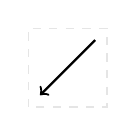
\begin{tikzpicture}
                \draw[white!90!black,dashed] (0,0) rectangle (1,1);
                \draw[thick,->] (0.85,0.85) -- (0.15,0.15);
            \end{tikzpicture}
        }
        \wrongchoice{
            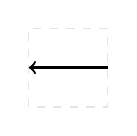
\begin{tikzpicture}
                \draw[white!90!black,dashed] (0,0) rectangle (1,1);
                \draw[thick,->] (1.0,0.5) -- (0.0,0.5);
            \end{tikzpicture}
        }
        \wrongchoice{
            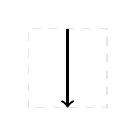
\begin{tikzpicture}
                \draw[white!90!black,dashed] (0,0) rectangle (1,1);
                \draw[thick,->] (0.5,1.0) -- (0.5,0.0);
            \end{tikzpicture}
        }
    \end{choices}
    \end{multicols}
\end{question}
}

\element{nysed}{
\begin{question}{June2016-Q11}
    The diagram below represents the electric field in the region of two small charged spheres,
    \begin{center}
    \begin{tikzpicture}
        %% NOTE: TODO: draw charge
        %% charge A
        \begin{scope}[xshift=-1cm]
            \node[draw,circle,minimum size=1cm] at (0,0) {$A$};
            \foreach \x in {18,54,90,126,162,198,234,270,306,342}
                \draw (\x,0) -- (\x,0);
        \end{scope}
        %% charge B
    \end{tikzpicture}
    \end{center}
    What is the sign of the net charge on $A$ and $B$?
    \begin{choices}
        \wrongchoice{$A$ is positive and $B$ is positive.}
        \wrongchoice{$A$ is positive and $B$ is negative.}
      \correctchoice{$A$ is negative and $B$ is negative.}
        \wrongchoice{$A$ is negative and $B$ is positive.}
    \end{choices}
\end{question}
}

\element{nysed}{
<<<<<<< HEAD
\begin{question}{June2016-Q18}
    A \SI{5.8e4}{\watt} elevator motor can lift a total weight of \SI{2.1e4}{\newton} with a maximum constant speed of:
    \begin{multicols}{2}
    \begin{choices}
        \wrongchoice{\SI{0.28}{\meter\per\second}}
        \wrongchoice{\SI{0.36}{\meter\per\second}}
      \correctchoice{\SI{2.8}{\meter\per\second}}
        \wrongchoice{\SI{3.6}{\meter\per\second}}
    \end{choices}
    \end{multicols}
\end{question}
}

\element{nysed}{
\begin{question}{June2016-Q19}
    A stationary police officer directs radio waves emitted by a radar gun at a vehicle moving toward the officer. 
=======
\begin{question}{June2016-Q19}
    A stationary police officer directs radio waves emitted by a radar gun at a vehicle moving toward the officer.
>>>>>>> develop
    Compared to the emitted radio waves,
        the radio waves reflected from the vehicle and received by the radar gun have a:
    \begin{choices}
        \wrongchoice{longer wavelength}
        \wrongchoice{higher speed}
        \wrongchoice{longer period}
      \correctchoice{higher frequency}
    \end{choices}
\end{question}
}

\element{nysed}{
\begin{question}{June2016-Q20}
    A light wave strikes the Moon and reflects toward Earth. 
    As the light wave travels from the Moon toward Earth,
        the wave carries:
    \begin{choices}
      \correctchoice{energy, only}
        \wrongchoice{matter, only}
        \wrongchoice{both energy and matter}
        \wrongchoice{neither energy nor matter}
    \end{choices}
\end{question}
}

\element{nysed}{
\begin{question}{June2016-Q25}
    In the diagram below, point $P$ is located in the electric field between two oppositely charged parallel plates.
    \begin{center}
    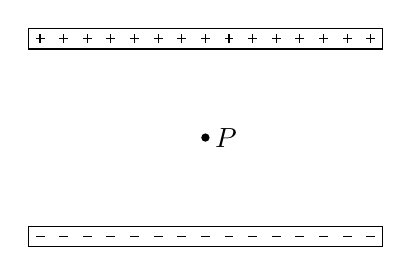
\begin{tikzpicture}[scale=0.75]
        %% point P
        \fill (3,1.5) circle (2pt) node[anchor=west] {$P$};
        %% Bottom negative
        \draw (0,0) rectangle (6,-1em);
        \foreach \x in {2,6,...,58}
            \foreach \y in {0,180} {
                \draw (\x mm,-0.5em) -- ++(\y:0.5ex);
            }
        %% Top positive
        \draw (0,3) rectangle (6,3cm+1em);
        \foreach \x in {2,6,...,58}
            \foreach \y in {0,90,180,270} {
                \draw (\x mm,3cm+0.5em) -- ++(\y:0.5ex);
            }
    \end{tikzpicture}
    \end{center}
    Compared to the magnitude and direction of the electrostatic force on an electron placed at point $P$,
    the electrostatic force on a proton placed at point $P$ has:
    \begin{choices}
        \wrongchoice{the same magnitude and the same direction}
      \correctchoice{the same magnitude, but the opposite direction}
        \wrongchoice{a greater magnitude, but the same direction}
        \wrongchoice{a greater magnitude and the opposite direction}
    \end{choices}
\end{question}
}

\element{nysed}{
\begin{question}{June2016-Q27}
    A gamma ray photon and a microwave photon are traveling in a vacuum. 
    Compared to the wavelength and energy of the gamma ray photon,
        the microwave photon has a:
    \begin{choices}
        \wrongchoice{shorter wavelength and less energy}
        \wrongchoice{shorter wavelength and more energy}
      \correctchoice{longer wavelength and less energy}
        \wrongchoice{longer wavelength and more energy}
    \end{choices}
\end{question}
}

\element{nysed}{
\begin{question}{June2016-Q32}
    A particle with a charge of \num{3.00} elementary charges moves through a potential difference of \SI{4.50}{\volt}.
    What is the change in electrical potential energy of the particle?
    \begin{multicols}{2}
    \begin{choices}
        \wrongchoice{\SI{1.07e-19}{\eV}}
        \wrongchoice{\SI{2.16e-18}{\eV}}
        \wrongchoice{\SI{1.50}{\eV}}
      \correctchoice{\SI{13.5}{\eV}}
    \end{choices}
    \end{multicols}
\end{question}
}

\element{nysed}{
\begin{question}{June2016-Q34}
    A transverse wave is moving toward the right in a uniform medium. 
    Point $X$ represents a particle of the uniform medium. 
    Which diagram represents the direction of the motion of particle $X$ at the instant shown?
    \begin{multicols}{2}
    \begin{choices}
        \AMCboxDimensions{down=-1.5em}
        %% NOTE: ANS is 3
        \wrongchoice{
            \begin{tikzpicture}
                %% NOTE: TODO: draw wave motion
            \end{tikzpicture}
        }
    \end{choices}
    \end{multicols}
\end{question}
}

\element{nysed}{
\begin{question}{June2016-Q35}
    Which diagram represents magnetic field lines between two north magnetic poles?
    \begin{multicols}{2}
    \begin{choices}
        \AMCboxDimensions{down=-1.5em}
        %% NOTE: ANS is 4
        \wrongchoice{
            \begin{tikzpicture}
                %% NOTE: TODO: draw magnets
            \end{tikzpicture}
        }
    \end{choices}
    \end{multicols}
\end{question}
}

%% Part B-1
\element{nysed}{
\begin{question}{June2016-Q40}
    Which graph represents the motion of an object traveling with a positive velocity and a negative acceleration?
    \begin{multicols}{2}
    \begin{choices}
        %% NOTE: TODO: make grpahs
        \AMCboxDimensions{down=-2.5em}
        %% NOTE: ANS is 2
        \wrongchoice{
            \begin{tikzpicture}
                \begin{axis}[
                    axis y line=left,
                    axis x line=bottom,
                    axis line style={->},
                    xlabel={time},
                    xtick=\empty,
                    ylabel={position},
                    ytick=\empty,
                    xmin=0,xmax=11,
                    ymin=0,ymax=11,
                    width=0.95\columnwidth,
                    very thin,
                ]
                \addplot[line width=1pt,domain=0:10]{8};
                \end{axis}
            \end{tikzpicture}
        }
    \end{choices}
    \end{multicols}
\end{question}
}


\element{nysed}{
\begin{question}{June2016-Q47}
    Parallel wave fronts are incident on an opening in a barrier. 
    Which diagram shows the configuration of wave fronts and barrier opening that will result in the greatest diffraction of the waves passing through the opening? 
    [Assume all diagrams are drawn to the same scale.]
    \begin{multicols}{2}
    \begin{choices}
        \AMCboxDimensions{down=-1.5em}
        %% NOTE: ANS is 2
        \wrongchoice{
            \begin{tikzpicture}
                %% NOTE: TODO: draw wave front
            \end{tikzpicture}
        }
    \end{choices}
    \end{multicols}
\end{question}
}

\element{nysed}{
\begin{question}{June2016-Q48}
    A singer demonstrated that she could shatter a crystal glass by singing a note with a wavelength of \SI{0.320}{\meter} in air at STP.
    What was the natural frequency of the glass?
    \begin{multicols}{2}
    \begin{choices}
        \wrongchoice{\SI{9.67e-4}{\hertz}}
        \wrongchoice{\SI{1.05e2}{\hertz}}
      \correctchoice{\SI{1.03e3}{\hertz}}
        \wrongchoice{\SI{9.38e8}{\hertz}}
    \end{choices}
    \end{multicols}
\end{question}
}

\element{nysed}{
\begin{question}{June2016-Q49}
    The diagram below represents a standing wave in a string.
    \begin{center}
    \begin{tikzpicture}
        %% NOTE: TODO: draw standing wave
    \end{tikzpicture}
    \end{center}
    Maximum constructive interference occurs at the:
    \begin{choices}
        \wrongchoice{antinodes $A$, $C$, and $E$}
        \wrongchoice{nodes $A$, $C$, and $E$}
      \correctchoice{antinodes $B$ and $D$}
        \wrongchoice{nodes $B$ and $D$}
    \end{choices}
\end{question}
}

\element{nysed}{
\begin{question}{June2016-Q50}
    Which circuit diagram represents voltmeter $V$ connected correctly to measure the potential difference across resistor $R_2$?
    \begin{choices}
        \AMCboxDimensions{down=-0.75cm}
        \ctikzset{bipoles/length=0.75cm}
        %% NOTE: TODO: finish circuits
        \wrongchoice{
            \begin{circuitikz}
                \draw (0,0) to [battery,l=\SI{12}{\volt}] (0,2) to (2,2)
                            to [R,l_=$R_1$] (4,2)
                            to [R,l=$R_2$] (4,0)
                            to [voltmeter] (0,0);
            \end{circuitikz}
        }
        \wrongchoice{
            \begin{circuitikz}
                \draw (0,0) to [battery,l=\SI{12}{\volt}] (0,2) to (2,2)
                            to [R,l_=$R_1$] (4,2)
                            to [R,l=$R_2$] (4,0);
                \draw (0,2) to [voltmeter] (2,2);
            \end{circuitikz}
        }
        \wrongchoice{
            \begin{circuitikz}
                \draw (0,0) to [battery,l=\SI{12}{\volt}] (0,2) to (1.3,2)
                            to [R,l=\SI{2}{\ohm}] (1.3,0) to (0,0);
                \draw (1.3,2) to (2.6,2)
                            to [R,l=\SI{2}{\ohm}] (2.6,0) to (1.3,0);
                \draw (2.6,2) to (4,2)
                            to [voltmeter] (4,0) to (2.6,0);
            \end{circuitikz}
        }
        %% NOTE: ANS is 3
    \end{choices}
\end{question}
}


<<<<<<< HEAD
=======

%% NOTE: electromagneticApplication?, 2dkinematics, electrostatics, Sound, light

%% Section June2015
%%--------------------
\element{nysed}{
\begin{question}{June2015-Q22}
    Which diagram best represents the position of a ball,
        at equal time intervals,
        as it falls freely from rest near Earth's surface?
    \begin{multicols}{2}
    \begin{choices}
        %% NOTE: make ticker tape graph
        \wrongchoice{
            \begin{tikzpicture}
                \draw[white] (0,0) rectangle (2,4);
                \draw[domain=0:10,samples=4,mark=*,only marks] plot ({1.0}, {0.02*\x*\x});
                \draw (0,0) -- (2,0) node[pos=0.5,anchor=north] {Earth's Surface};
            \end{tikzpicture}
        }
        \wrongchoice{
            \begin{tikzpicture}
                \draw[white] (0,0) rectangle (1,-4);
                \draw[domain=0:10,samples=4,mark=*,only marks] plot ({1.0}, {-0.02*\x*\x});
                \draw (0,-4) -- (2,-4) node[pos=0.5,anchor=north] {Earth's Surface};
            \end{tikzpicture}
        }
        \wrongchoice{
            \begin{tikzpicture}
                \draw[white] (0,0) rectangle (1,-4);
                \draw[domain=0:10,samples=4,mark=*,only marks] plot ({1.0}, {0.2*\x});
                \draw (0,0) -- (2,0) node[pos=0.5,anchor=north] {Earth's Surface};
            \end{tikzpicture}
        }
        \wrongchoice{
            \begin{tikzpicture}
                \draw[white] (0,0) rectangle (1,-4);
                \draw[domain=0:10,samples=4,mark=*,only marks] plot ({1.0}, {0.04*(10-\x)*\x});
                \draw (0,0) -- (2,0) node[pos=0.5,anchor=north] {Earth's Surface};
            \end{tikzpicture}
        }
    \end{choices}
    \end{multicols}
\end{question}
}

%% NOTE: TODO: finish next two questions
\newcommand{\JuneTwentyFifteenQThirty}{
    \begin{tikzpicture}
    \end{tikzpicture}
}

\element{nysed}{
\begin{question}{June2015-Q30}
    %Base your answers to questions 30 and 31 on the diagram
    %    below and on your knowledge of physics. 
    The diagram represents two small, charged,
        identical metal spheres, $A$ and $B$ that are separated
        by a distance of \SI{2.0}{\meter}.
    \begin{center}
        \JuneTwentyFifteenQThirty
    \end{center}
    What is the magnitude of the electrostatic force exerted by sphere A on sphere B?
    \begin{multicols}{2}
    \begin{choices}
        \wrongchoice{\SI{7.2e-3}{\newton}}
        \wrongchoice{\SI{3.6e-3}{\newton}}
        \wrongchoice{\SI{8.0e-13}{\newton}}
        \wrongchoice{\SI{4.0e-13}{\newton}}
    \end{choices}
    \end{multicols}
\end{question}
}

\element{nysed}{
\begin{question}{June2015-Q31}
    The diagram represents two small, charged,
        identical metal spheres, $A$ and $B$ that are separated
        by a distance of \SI{2.0}{\meter}.
    \begin{center}
        \JuneTwentyFifteenQThirty
    \end{center}
    If the two spheres were touched together and then separated,
        the charge on sphere $A$ would be
    \begin{multicols}{2}
    \begin{choices}
        \wrongchoice{\SI{-3.0e-7}{\coulomb}}
        \wrongchoice{\SI{-6.0e-6}{\coulomb}}
        \wrongchoice{\SI{-1.3e-6}{\coulomb}}
        \wrongchoice{\SI{-2.6e-6}{\coulomb}}
    \end{choices}
    \end{multicols}
\end{question}
}

\element{nysed}{
\begin{question}{June2015-Q32}
    The horn of a moving vehicle produces a sound of constant frequency. 
    Two stationary observers, $A$ and $C$,
    and the vehicle's driver, $B$, positioned as represented
        in the diagram below, hear the sound of the horn.
    \begin{center}
        %% NOTE: insert graphic
        %\includegraphics[width=0.9\columnwidth,keepaspectratio]{June2015-Q32}
    \end{center}
    Compared to the frequency of the sound of the horn heard by driver $B$,
        the frequency heard by observer $A$ is:
    \begin{choices}
        \wrongchoice{lower and the frequency heard by observer $C$ is lower}
        \wrongchoice{lower and the frequency heard by observer $C$ is higher}
        \wrongchoice{higher and the frequency heard by observer $C$ is lower}
        \wrongchoice{higher and the frequency heard by observer $C$ is higher}
    \end{choices}
\end{question}
}

\element{nysed}{
\begin{question}{June2015-Q34}
    The diagram below shows a ray of monochromatic light
        incident on a boundary between air and glass.
    \begin{center}
    \begin{tikzpicture}
        %% NOTE:
    \end{tikzpicture}
    \end{center}
    Which ray best represents the path of the reflected light ray?
    \begin{multicols}{4}
    \begin{choices}[o]
        \wrongchoice{$A$}
        \wrongchoice{$B$}
        \wrongchoice{$C$}
        \wrongchoice{$D$}
    \end{choices}
    \end{multicols}
\end{question}
}


>>>>>>> develop
\endinput

